\documentclass[11pt]{article}
\usepackage[top=5pt,bottom=5pt,left=20pt,right=20pt]{geometry}
\usepackage{calc}
\usepackage{tikz,pgf}
\usetikzlibrary{shapes,shadows}
\usepackage[english]{babel}
\usetikzlibrary{backgrounds}
\usepackage[colorlinks=true,allcolors=black,breaklinks=true]{hyperref}
\usepackage{color}
\usepackage{xcolor}
\usepackage{array}
\usepackage{graphics}
\usepackage{titlesec}
% fonts
\usepackage{fontawesome5}
\usepackage{academicons}

\usepackage[sfdefault]{ClearSans}

% page style
\pagestyle{empty}
\setcounter{secnumdepth}{0}
\parindent=0pt

% Top banner background
\colorlet{banerColor}{gray!10}
%\definecolor{SwishLineColour}{HTML}{007ae0}
\definecolor{mauveClair}{RGB}{204,153,255}
\definecolor{mauveMoyen}{RGB}{153,102,204}

\newcommand{\drawBaner}{%
	\begin{tikzpicture}[remember picture, overlay]
		\fill[banerColor] (-30pt,30pt) rectangle (\paperwidth,-0.115\paperheight);
	\end{tikzpicture}%
}
\newcommand{\liner}{\begin{tikzpicture}[remember picture,overlay]%\
		\fill[left color=mauveClair, right color=white,white] (0,-0.5pt) rectangle (\linewidth,-2pt);
		\end{tikzpicture}}
%\titleformat{command}[shape]{format}{label}{sep}{before-code}[after-code]
\titleformat{\section}[display]{\Large\bfseries}{}{0pt}{\liner}[\vspace*{-5pt}]

\newcommand{\slink}[1]{\underline{\smash{\color[RGB]{153,102,204}#1}}}
\newcommand{\link}[1]{\href{#1}{\color[RGB]{153,102,204}\faGlobe}}



\newcommand{\cvInfo}[2]{\makebox[1em]{\color{black}#1} \color{black}#2\hspace*{1em}}

\newcommand{\cvEduc}[3]{\begin{tabular}{>{\raggedleft\arraybackslash}p{3cm}>{\raggedright\arraybackslash}p{\linewidth}}
		#1 & \textbf{#2}  \\
		&#3 \\
\end{tabular}
\vspace*{3pt}}

\newcommand{\cvWP}[4]{\begin{tabular}{>{\raggedleft\arraybackslash}p{3cm}>{\raggedright\arraybackslash}p{13cm}>{\raggedleft\arraybackslash}m{3cm}}%
		#1 & \textbf{#2} & \textbf{#3}  \\%
		&\multicolumn{2}{>{\raggedright\arraybackslash}p{16cm}}{#4} \\%
\end{tabular}}

\newcommand{\cvitem}[2]{\begin{tabular}{>{\raggedleft\arraybackslash}p{3cm}>{\raggedright\arraybackslash}p{16cm}}
		\textbf{#1} & #2  \\
\end{tabular}}

\newcommand{\cvitemi}[2]{\begin{tabular}{>{\raggedleft\arraybackslash}p{3cm}>{\raggedright\arraybackslash}p{16cm}}
		#1 & #2  \\
	\end{tabular}}


\newcommand{\cvRefTitle}[2]{\begin{tabular}{>{\raggedleft\arraybackslash}p{3cm}>{\raggedright\arraybackslash}p{16cm}}
		 & \textbf{#1} $|$ \textbf{#2}  \\
\end{tabular}}

\newcommand{\cvRefEntry}[1]{\begin{tabular}{>{\raggedleft\arraybackslash}p{3cm}>{\raggedright\arraybackslash}p{16cm}}
		& #1 \\
\end{tabular}}


\title{Curriculum Vitae}
\author{Anna Stefano Narivelomanana}

\newcommand{\header}{
	\newpage
	\vspace*{10pt}
	\begin{tikzpicture}[remember picture,overlay]%\
		\node at (0pt,0) [right] {Anna Stefano Narivelomanana};
		\node at (\linewidth,0) [left]{Curriculum Vitae};
		\fill[left color=gray,right color=gray,white] (0,-5pt) rectangle (\linewidth,-6pt);
	\end{tikzpicture}
	\vspace*{10pt}}

\begin{document}
\drawBaner

\begin{minipage}{\linewidth}
	\begin{center}
		\bfseries
		Anna Stefano NARIVELOMANANA 
		%Mathematician/ Teacher / Python developer
	\end{center}
	\hfil\begin{minipage}{0.65\linewidth}
		\cvInfo{\faUser}{Born in 7 April 1998, Ambohidratrimo, Antananarivo, Madagascar}

		\cvInfo{\faHome}{Logt 146 cité Akany Firaisana Antananarivo}

		%\cvInfo{\faHome}{P.O BOX  608,Crystal Gardens, Limbe Cameroon}

		\cvInfo{\faEnvelope}{\slink{\href{anna.narivelomanana@aims-cameroon.org}{\slink{anna.narivelomanana@aims-cameroon.org}}}}
		
		Homepage:{\slink{\href{https://nanasteff.github.io/}{\slink{nanasteff.github.io/}}}}
		
		%\href{https://nanasteff.github.io/}{nanasteff.github.io}
		
		%Homepage : {\slink{nanasteff.github.io/}}
	\end{minipage}\begin{minipage}{0.7\linewidth}
		\cvInfo{\faPhone}{\ttfamily+261 348 189 668}(Signal)

		\cvInfo{\faGithub}{\slink{\href{https://github.com/NanaSteff}{\slink{NanaSteff}}}}

		\cvInfo{\faLinkedin}
		{\slink{\href{https://www.linkedin.com/in/anna-stefano-narivelomanana-86a995269/}{\slink{Anna Stefano Narivelomanana}}}}

		\cvInfo{\faEnvelope}{\slink{\href{mailto:annanarivelomanana07@gmail.com}{\slink{annanarivelomanana07@gmail.com}}}}
	\end{minipage}\hfil
\end{minipage}

%\section{Summary}
%I am a student in mathematics with a strong interest in information security. I am very interested in maths generally based in the field of cryptography, algebra and number theory, and also in computing. Currently, I am a new graduate from AIMS Cameroon, and I did a master's thesis on the stream cipher family of cryptography. I am self-taught in programming with Python 3, generally based on Gérard Swinnen's book, and am currently very passionate about computing technologies. I am motivated, dynamic, serious, and creative, and I am a problem solver.

%I am a recent mathematics graduate from AIMS Cameroon. I am interested in security and privacy. Currently, I completed a 3 weeks intensive bootcamp program offered by Tech4dev providing an introduction to cybersecurity. I have taken cryptography courses and my Master's thesis at AIMS focused on stream ciphers and the Berlekamp-Massey algorithm under the supervision of Dr. Giulio Codogni from Tor Vergata University of Roma. I explored algebraic techniques for constructing and breaking stream cipher cryptosystems. I have strong Python programming skills and practical experience with RSA encryption. I use Git and GitHub for version control. I am comfortable with Linux and completed a web development bootcamp where I created my own portfolio. 

%I graduated with a Master's degree in Fundamental Mathematics from AIMS Cameroon in June 2023. As part of my degree requirement, I competed a thesis on Stream Cipher Cryptography and the Berlekamp-Massey algorithm under the supervision of Dr. Giulio Codogni from Tor Vergata University of Roma. I explored an algebraic techniques for constructing and breaking stream cipher cryptosystems. I have a strong Python programming skills and practical experience with RSA encryption. I use Git and GitHub for version control. I am comfortable with Linux and completed a web development bootcamp where I created my own portfolio.

\section{Education}
\cvEduc{2022 -- 2023}{Structured Master, Fundamental Science Stream}{African Institute of Mathematical Science Cameroon.}

\cvEduc{2020 -- 2022}{Master 1, in Mathematical Education}{Ecole Normale Supérieure, University of Antananarivo, Madagascar.}

\cvEduc{2016 -- 2020}{Bachelor degree, in Mathematical Education}{Ecole Normale Supérieure, University of Antananarivo, Madagascar.}

\cvEduc{2014 -- 2015}{Baccalauréat, série C}{Lycée Joseph Ravoahangy Andrianavalona Antananarivo, Madagascar.}

\section{Conference}
\cvWP{19 Feb. 2025}{1st Microarchitecture Security Conference}{}{Ruhr University, Bochum, Germany}

\section{Internships}
\cvEduc{Mar 2024 -- Feb 2025}{Research Internship on Multivariate-based Post-Quantum Cryptography Implementation}{Max Planck Institute for Security and Privacy, Bochum, Germany}

\cvWP{Jan.-Feb. 2020}{Mathematics Teaching Internship}{Course of study}{CEG 67Ha Betsimitatatra.}

\section{Schools}

\cvWP{Jun 2024}{Summer School on Real-World Crypto and Privacy 2024}{MPI-SP}{Vodice, Croatia}

\cvWP{Dec 2023}{Research School on Post-Quantum Cryptography}{CIMPA School}{Pondicherry University, India}

\section{Project and work}
\cvWP{2023}{Research~on~advanced~stream~cipher~cryptography}{AIMS Cameroon}{Supervised by Dr. Giulio Codogni, University of Roma Tor Vergata.}

\cvWP{2023}{Personal website \link{https://nanasteff.github.io/}}{Personal project}{An portfolio written in html, JavaScript and Bootstrap}

\cvWP{2023}{Berlekamp-Massey Algorithm \link{https://github.com/NanaSteff/Berlekamp_Massey_Algorithm}}{Personal project}{An implementation of the Berlekamp-Massey Algorithm  written in Python3 using Sympy.}

\cvWP{2023}{SPN Code \link{https://github.com/NanaSteff/Substitution_Permutation_Network_code}}{Personal project}{Encryption and decryption with Substitution Permutation Network written in Python3}

\cvWP{2023}{RSA cryptosystem \link{https://github.com/NanaSteff/Tkinter_RSA_code} }{Personal project}{A graphical interface for the RSA cryptosystem (encryption and decryption) made with Python3/Tkinter.}

%\cvWP{2022}{Olympic flag \link{https://github.com/NanaSteff/olympique_flag}}{Personal project}{It's a drawing of the Olympic flag on the python graphical interface Tkinter.}
%
\header
\section{Extra training}
\cvEduc{Sept-Oct 2023}{Cybersecurity bootcamp by Women Techsters}{HashCheck, Zphisher, John The Ripper.}
\cvEduc{June 2022}{Initiation to website development at Orange Digital Center Madagascar}{Html, CSS, MySQL, PHP.}

%\header

%\section{Extra activities}

%\cvEduc{June 2022}{Member of a tree data collection team in a forest}{Mantadia Park, Andasibe, Madagascar}

%\cvEduc{May 2022}{Sharing session about algorithm and initiation to Python programming}{Y-Tech club at YMCA Madagascar}

\section{Skills}
\cvitem{Languages}{Malagasy, English, French, German (low intermediate), Python, R, \LaTeX, SageMath.}

%\cvitem{Coding}{Python, R, \LaTeX, SageMath.}

\cvitem{Libraries}{Pandas, Numpy, Scipy, Sympy.}

\section{Extracurricular}
\cvEduc{June 2022}{Member of a tree data collection team in a forest}{Mantadia Park, Andasibe, Madagascar}

\cvEduc{May 2022}{Sharing session about algorithm and initiation to Python programming}{Y-Tech club at YMCA Madagascar}

\cvEduc{2023}{Leader of give-back team which mentors children in S.T.E.M.}{Save the Children Orphanage,
	 Limbe, Cameroon.}

\cvEduc{Clubs}{Gender and library clubs member at AIMS Cameroon.}

\cvEduc{Feb.-Jun. 2022}{Y-Tech club member at YMCA Madagascar}

%\cvitem{Other}{Singing, swimming, walking in the forest and exploring nature.}

\section{References}

\cvRefTitle{Dr. Peter Schwabe}{Scientific Director}

\cvRefEntry{Max Planck Institute for Security and Privacy}

%\cvRefEntry{Universitätsstraße 140, 44799 Bochum, Germany}

\cvRefEntry{Homepage : \href{https://cryptojedi.org/peter/index.shtml}{\color{mauveMoyen}\underline{https://cryptojedi.org/peter/index.shtml}}}

\cvRefEntry{Email: \href{mailto:peter@cryptojedi.org}{\color{mauveMoyen}\underline{peter@cryptojedi.org}}}
%%%%%%%%%%%%%%%%%%%%%%%%%%%%%%%%%%%%%%%

\vspace*{15pt}

\cvRefTitle{Dr. Giulio Codogni}{Professor of Mathematics and Cryptography}

%\cvRefEntry{Department of Mathematics}

\cvRefEntry{University of Rome Tor Vergata}

%\cvRefEntry{Street of Scientific Research 1, 00133 Rome, Italy}

\cvRefEntry{Homepage : \href{https://sites.google.com/view/giuliocodogni/home-page?authuser=0}{\color{mauveMoyen}\underline{https://sites.google.com/view/giuliocodogni/home-page?authuser=0}}}

%\cvRefEntry{Phone: +49 761 203 5830}

%\cvRefEntry{Fax: +49 761 203 5967}

\cvRefEntry{Email: \href{mailto:codogni@mat.uniroma2.it}{\color{mauveMoyen}\underline{codogni@mat.uniroma2.it}}}
%%%%%%%%%%%%%%%%%%%%%%%%%%%%%%%%%%%%%%%

\vspace*{15pt}
\cvRefTitle{Dr. Andreas Buchleitner}{Professor of Theoretical Physics}

%\cvRefEntry{Department for Quantum Optics and Statistics}

\cvRefEntry{Institute of Physics, Albert-Ludwigs-Universität Freiburg}

%\cvRefEntry{Hermann-Herder-Str. 3, D-79104 Freiburg}

\cvRefEntry{Homepage : \href{https://quantum.uni-freiburg.de/}{\color{mauveMoyen}\underline{https://quantum.uni-freiburg.de/}}}

%\cvRefEntry{Phone: +49 761 203 5830}

%\cvRefEntry{Fax: +49 761 203 5967}

\cvRefEntry{Email: \href{mailto:a.buchleitner@physik.uni-freiburg.de}{\color{mauveMoyen}\underline{a.buchleitner@physik.uni-freiburg.de}}}
%%%%%%%%%%%%%%%%%%%%%%%%%%%%%%%%%%%%%%%

\vspace*{15pt}
\cvRefTitle{Dr. Fortunat Rajaona Solofomampionona}{Research Fellow}

%\cvRefEntry{Department of Computer Science}

\cvRefEntry{Faculty of Engineering and Physical Sciences University of Surrey
}

%\cvRefEntry{Guildford GU2 7XH, Surrey, United Kingdom}

\cvRefEntry{Homepage : \href{https://sfrajaona.github.io/home.html}{\color{mauveMoyen}\underline{https://sfrajaona.github.io/home.html}}}

%\cvRefEntry{Phone: +49 761 203 5830}

%\cvRefEntry{Fax: +49 761 203 5967}

\cvRefEntry{Email: \href{mailto:s.rajaona@surrey.ac.uk}{\color{mauveMoyen}\underline{s.rajaona@surrey.ac.uk}}}
\end{document}
